\section{Part II}\label{P2}

In contrast to the first portion, this section does not come with the correspondences already provided. By utilizing the \texttt{findMatches} function, the objective is to locate the points that relate to each other first. Because this function could find a great number of points, a significant number of them could be incorrect or noisy. Consequently, the inliers, or the matches that are correct, ought to be communicated. The subsequent phase is analogous to the first step, which is to compute the "A" matrix and the fundamental matrix $F$, and then to locate epipolar lines together with the points that correspond to them after they have been normalized.

Getting back to the problem of identifying matching points, there are a few different approaches to obtain them, such as the Normalized Cross-Correlation (NCC) and the Scale-Invariant Feature Transform (SIFT). While SIFT will locate a large number of comparable points, it is important to note that not all of these points are inliers. For the purpose of filtering the correspondences, putting the outliers aside, and calculating the optimal fundamental matrix, the RANSAC (RANdom SAmpling Consensus) approach is utilized. This method chooses a few pairs of corresponding points at random from the points that were discovered by the \texttt{findMatches} function. These pairs are then used in the \texttt{EightPointsAlgorithmN(P1, P2)} function, which locates the fundamental matrix $F$, computes the $X^TFX$, which can be considered as the error (we considered the absolute value of $X^TFX$ for testing the fundamental matrix), and establishes a threshold. In this procedure, the outliers are identified, the inliers are retained, and the process is repeated for a significant number of repetitions. A change is also made to the total number of iterations. Whenever a superior fundamental matrix $F$ is discovered, the one that was previously used will be substituted for it. 

Now, there ought to be proper inlier pair points that appear to be accurate, and the error ought to be very close to zero; hence, the threshold ought to be getting smaller. In the end, one accurate $F$ would be discovered, along with the points that corresponded to it the best. When it was first implemented, the \texttt{findMatch} algorithm was utilized in conjunction with two distinct NCC and SIFT approaches. During the simulation of the code, it appeared that the NCC algorithm was unable to locate any matches in the two photos by employing the delta and sigma values of 5 and 10, respectively. Changing the values of these two factors and attempting to discover the appropriate value while taking into consideration the photographs is one approach that may be taken to try to solve this problem. In an effort to reduce the quantity of sigma, which represents the contribution of the Euclidian distance, and delta, which represents the size of the patch for the NCC technique, we made multiple attempts. This is Figure 5, which displays the findings for the scenario in which sigma and delta are equal to 5 and 4, respectively. In spite of the fact that the algorithm has been successful in locating matches using this method, it is immediately apparent that the matches are not accurate in any way, and flaws can be observed just by looking at the photographs. 

When it came to the SIFT approach, I had the same issue. This method uses a value for the comparison of the vectors that is equal to 0.4 for this particular example. This value is referred to as the sigma. In addition, the outcomes of this particular example are displayed in Figure 6. For the second time, it is clear that this method does not display correct matches in the same way that the NCC method does. At first glance, the results of NCC appeared to be more plausible than those of SIFT because the error was lower. There were other checks made on other values for the parameters that were given. It was not possible to find appropriate matches in any of the circumstances.

\begin{figure} [h]
    \centering
    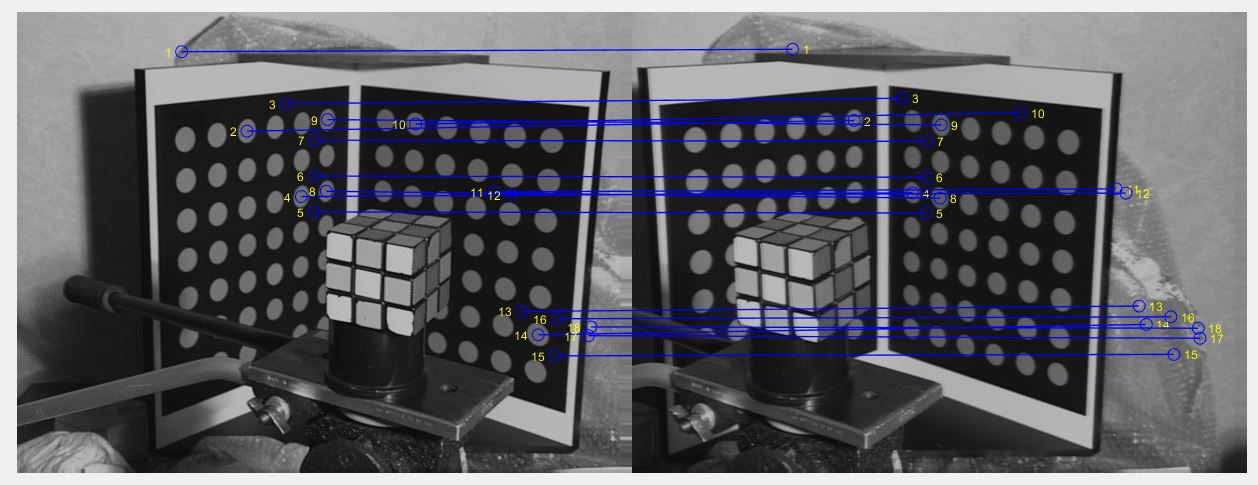
\includegraphics[width = \textwidth]{Resources/F5.jpg}
    \caption{Rubik correspondence points finding algorithm using NCC}
    \label{fig:Rubik correspondence points finding algorithm using NCC}
\end{figure}

\begin{figure} [ht]
    \centering
    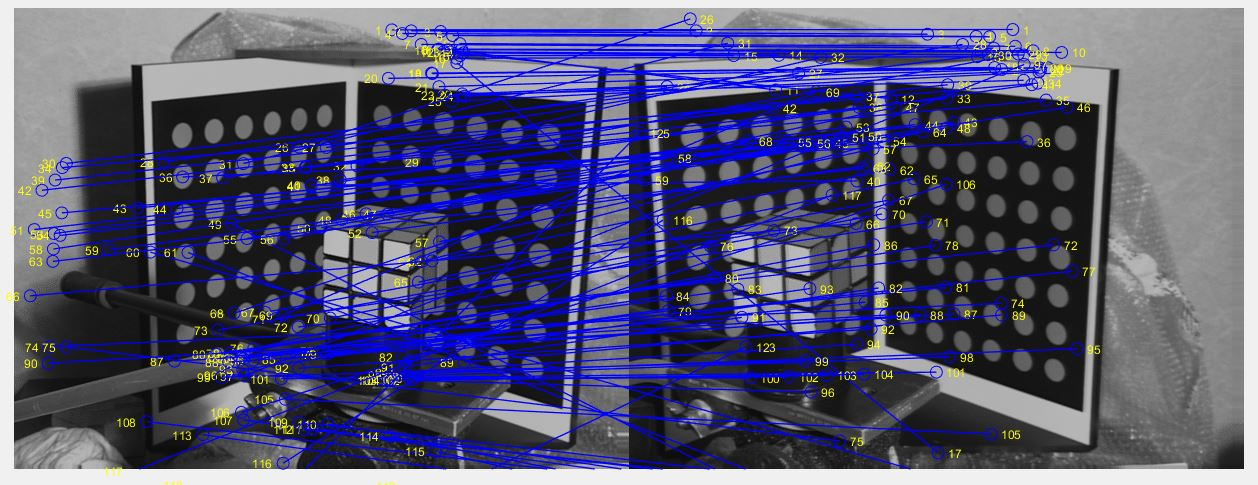
\includegraphics[width = \textwidth]{Resources/F6.jpg}
    \caption{Rubik correspondence points finding algorithm using Sift}
    \label{fig:Rubik correspondence points finding algorithm using Sift}
\end{figure}


The \texttt{Ransac} function was finished before moving on to the following step. The \texttt{ransac} function received the matches that were discovered in the previous section as inputs. These matches were delivered to the function. There is also a threshold that is defined here, and it is equal to 0.1 for the image that is being represented. Because the \texttt{Ransac} function had access to a greater number of correspondence points and the ability to select a variety of random points, it was given the SIFT method's correspondence points. The absolute value of the expression $X^TFX$ would be considered the test function or the error, according to the definition.

Figure 7 demonstrates that the fundamental matrix that has been optimized is not accurate since the epipolar lines are not shown in the correct manner. The reason for this is primarily due to the fact that the \texttt{Ransac} function is an optimization method, and if the inputs are incorrect, then the optimization and the optimal fundamental matrices will also be incorrect. In order to function properly, RANSAC is predicated on the premise that the majority of the data points are inliers and that the model should be able to adequately fit these inliers. If a substantial number of incorrect matches are provided, the algorithm may attempt to fit the model to these outliers rather than the actual underlying model, which will result in the generation of an incorrect model because of this. Due to the presence of noise and complexity in the photographs, the majority of the matches that were discovered for this collection of pictures, which can also be seen in Figure 6, are incorrect. As a result of this issue, the \texttt{Ransac} function produces incorrect resulting values.

\begin{figure} [ht]
    \centering
    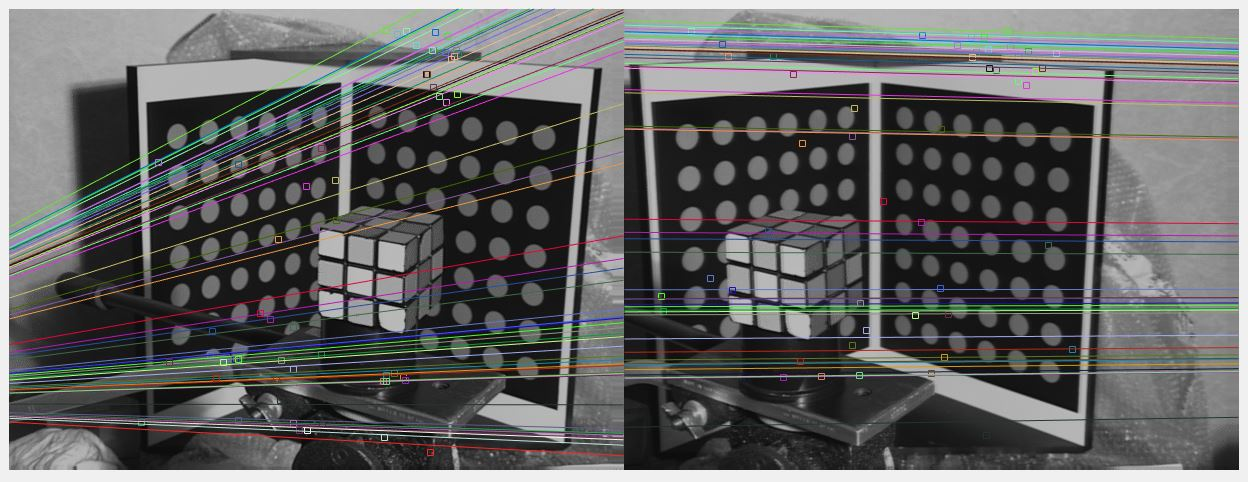
\includegraphics[width = \textwidth]{Resources/F7.jpg}
    \caption{Rubik correspondence points finding algorithm using Sift}
    \label{fig:Rubik correspondence points finding algorithm using Sift - 2}
\end{figure}

It is possible to see that the values of the epipolar constraint expression ($X^TFX$) for the output points of the \texttt{Ransac} function are actually very close to zero. This indicates that the \texttt{Ransac} function has been successful in locating an optimized fundamental matrix; however, there are some matches that are not recognized in the correct manner. In spite of the fact that the epipolar constraint is tested on both the left and right epipoles, the result is quite near to zero. In order to lessen the effect that incorrect matches have on RANSAC, it is essential to preprocess and filter the data with great care before applying the algorithm.

It is written in the \texttt{Main2} MATLAB script that the primary script for this portion is constructed. For the purpose of observing the results concerning the relevant set of photographs, all that is required is to change or remove the comment from the names of the input images. It should be brought to your attention that the \texttt{findMatches} function, which has a significant impact on the outputs, can be used with a variety of values, depending on the image being analyzed. For these arguments, there are also some values that have been tested and commented on within the \texttt{findMatches} method.